% This file was created with tikzplotlib v0.10.1.
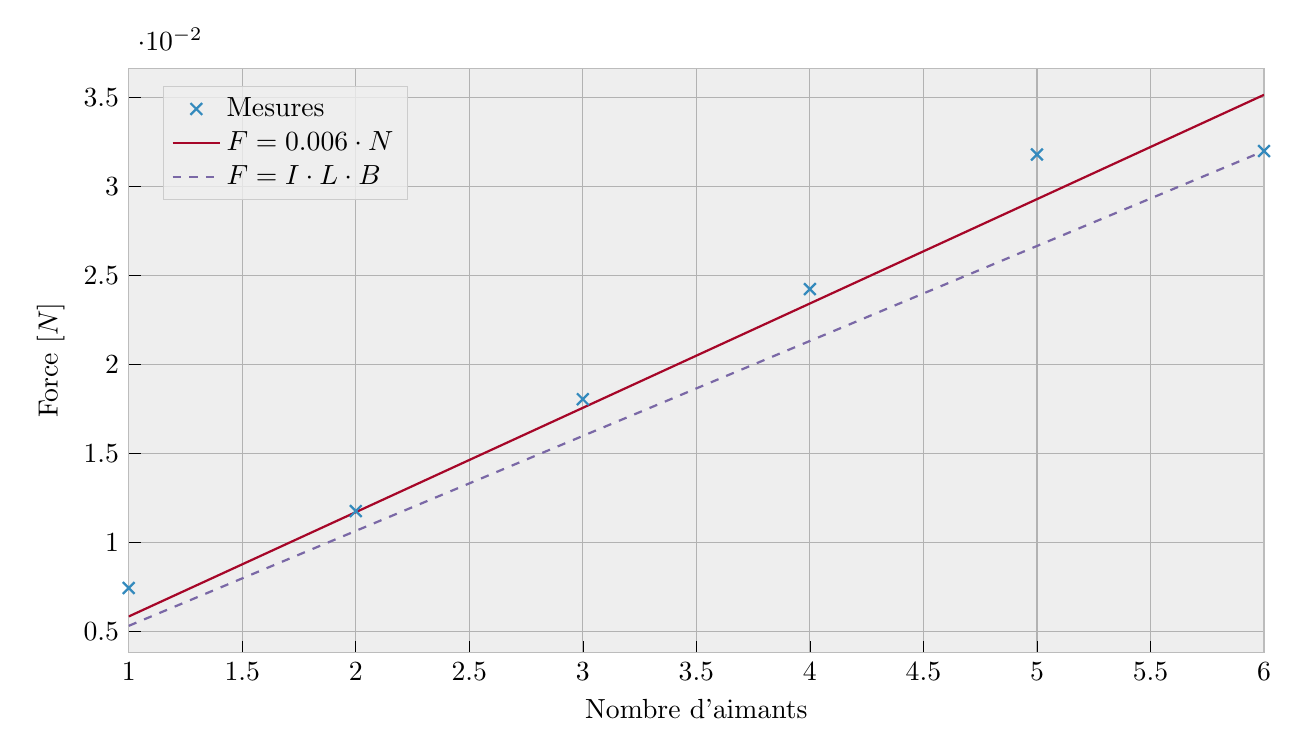
\begin{tikzpicture}

\definecolor{darkgray178}{RGB}{178,178,178}
\definecolor{firebrick166640}{RGB}{166,6,40}
\definecolor{lightgray204}{RGB}{204,204,204}
\definecolor{silver188}{RGB}{188,188,188}
\definecolor{slategray122104166}{RGB}{122,104,166}
\definecolor{steelblue52138189}{RGB}{52,138,189}
\definecolor{whitesmoke238}{RGB}{238,238,238}

\begin{axis}[
axis background/.style={fill=whitesmoke238},
axis line style={silver188},
height=9cm,
legend cell align={left},
legend style={
  fill opacity=0.8,
  draw opacity=1,
  text opacity=1,
  at={(0.03,0.97)},
  anchor=north west,
  draw=lightgray204,
  fill=whitesmoke238
},
tick pos=left,
width=16cm,
x grid style={darkgray178},
xlabel={Nombre d'aimants},
xmajorgrids,
xmin=1, xmax=6,
xtick style={color=black},
y grid style={darkgray178},
ylabel={Force \(\displaystyle [N]\)},
ymajorgrids,
ymin=0.00383986038526585, ymax=0.0366251319094172,
ytick style={color=black}
]
\addplot [thick, steelblue52138189, mark=x, mark size=3, mark options={solid}, only marks]
table {%
1 0.00745558738708496
2 0.0117720365524292
3 0.0180504322052002
4 0.0242307186126709
5 0.0317844152450562
6 0.0319806337356567
};
\addlegendentry{Mesures}
\addplot [thick, firebrick166640]
table {%
1 0.00585579872131348
6 0.0351349115371704
};
\addlegendentry{$F = 0.006 \cdot N$}
\addplot [thick, slategray122104166, dashed]
table {%
1 0.00533008575439453
6 0.0319806337356567
};
\addlegendentry{$F = I \cdot L \cdot B$}
\end{axis}

\end{tikzpicture}
